\chapter{Transformer}

\section{Introduzione al Meccanismo di Attenzione}
I \textbf{Transformer} rappresentano una delle innovazioni più significative e rivoluzionarie nell'ambito del Deep Learning. Essi si basano su un paradigma di elaborazione fondamentale noto come \textbf{attenzione} (\textit{attention}), il quale consente a una rete neurale di assegnare pesi differenti e dinamici a diversi elementi di input. A differenza delle reti neurali tradizionali (come i perceptroni multistrato o le reti convoluzionali), in cui i pesi sinaptici moltiplicano le attivazioni e rimangono fissi una volta completato l'addestramento, il meccanismo di attenzione calcola dei coefficienti di ponderazione le cui magnitudo \emph{dipendono direttamente dai valori degli input specifici} elaborati al momento dell'inferenza.

Questa proprietà permette di catturare potenti \emph{bias induttivi} (\textit{inductive biases}) legati a strutture di dati sequenziali e non strutturate. Il termine stesso ``Transformer'' deriva dalla funzione intrinseca dell'architettura: trasformare un insieme di vettori situati in un dato spazio di rappresentazione in un corrispondente insieme di vettori, aventi la medesima dimensionalità, collocati in un nuovo spazio di rappresentazione caratterizzato da una struttura semantica più ricca e meglio adattabile a compiti a valle (\textit{downstream tasks}).

\begin{observation}{Flessibilità della Struttura di Input}
Gli input di un Transformer non sono vincolati a griglie rigide bidimensionali (come nelle immagini per le CNN) o a catene strettamente sequenziali orientate nel tempo (come nelle RNN). Essi possono assumere la forma di insiemi non strutturati di vettori, sequenze ordinate o grafi, garantendo un'ampia genericità applicativa.
\end{observation}

\subsection{Origini Storiche e Vantaggi Architetturali}
Il concetto di attenzione fu originariamente introdotto come estensione delle reti neurali ricorrenti (RNN) per il miglioramento della traduzione automatica (Bahdanau et al., 2014). Tuttavia, Vaswani et al. (2017) hanno dimostrato che è possibile eliminare completamente la struttura ricorrente, focalizzandosi esclusivamente sul meccanismo di attenzione.

L'architettura Transformer presenta evidenti vantaggi rispetto ai modelli precedenti:
\begin{enumerate}
    \item \textbf{Efficacia del Transfer Learning e Modelli di Fondazione:} Un modello Transformer può essere pre-addestrato su enormi moli di dati non etichettati tramite apprendimento auto-supervisionato (\textit{self-supervised learning}) e successivamente adattato (\textit{fine-tuned}) a molteplici compiti specifici. Tali modelli generici sono noti come \textbf{modelli di fondazione} (\textit{foundation models}).
    \item \textbf{Ipotesi di Scaling (\textit{Scaling Hypothesis}):} Sostiene che il semplice incremento della scala del modello (misurato dal numero di parametri apprendibili) e del dataset di addestramento conduca a continui e significativi miglioramenti delle prestazioni, senza la necessità di apportare modifiche architetturali.
    \item \textbf{Parallelismo Massivo su Hardware Moderno:} Rimuovendo le dipendenze temporali sequenziali tipiche delle RNN, i Transformer consentono un'elaborazione altamente parallela su architetture hardware dedicate come le GPU e le TPU.
\end{enumerate}

\begin{definition}{Esempio Applicativo non Linguistico: Modellazione Proteica}
Un esempio illuminante dell'efficacia dell'attenzione generalizzata riguarda la biologia strutturale. Una proteina può essere vista come una sequenza monodimensionale di amminoacidi. Nella cellula, la proteina si ripiega in una struttura tridimensionale complessa dove amminoacidi distanti nella sequenza 1D diventano spazialmente contigui nel 3D. Il meccanismo di attenzione permette a elementi lontani nella sequenza di ``prestare attenzione'' l'uno all'altro, consentendo di predirne la struttura tridimensionale con elevata precisione.
\end{definition}

\section{Elaborazione nei Transformer (\textit{Transformer Processing})}
Definiamo formalmente il modello matematico di elaborazione dati all'interno di un Transformer.

\begin{definition}{Token e Feature}
Sia data una collezione di $N$ vettori di input $x_1, x_2, \dots, x_N$, ciascuno di dimensionalità $D$, ovvero $x_n \in \mathbb{R}^D$ per $n = 1, \dots, N$. Tali vettori di dati prendono il nome di \textbf{token}. Gli elementi individuali $x_{ni}$ dei vettori $x_n$ prendono il nome di \textbf{feature}.
\end{definition}

A seconda del dominio applicativo, un token può rappresentare:
\begin{itemize}
    \item Una parola o sotto-parola all'interno di una frase;
    \item Una \textit{patch} quadrata di pixel all'interno di un'immagine;
    \item Un amminoacido all'interno di una catena proteica.
\end{itemize}
Il grande vantaggio dei Transformer risiede nella capacità di unificare e combinare tipi di dati eterogenei all'interno di un unico insieme congiunto di token.



\subsection{Tokenizzazione ed embedding iniziale}

Prima di essere elaborato dal Transformer, il testo viene suddiviso in una sequenza di token. Un token può corrispondere a una parola, a una parte di parola o, in generale, a una sequenza di caratteri, a seconda del metodo di tokenizzazione adottato. A ciascun token viene associato un identificativo intero, che permette di rappresentarlo all'interno del vocabolario del modello.

Gli identificativi dei token vengono successivamente convertiti in vettori reali attraverso una matrice di embedding apprendibile. Indicando con $V$ la dimensione del vocabolario e con $D$ la dimensione dello spazio degli embedding, tale matrice può essere definita come

$$
E \in \mathbb{R}^{V \times D}.
$$

La matrice $E$ contiene gli embedding iniziali dei $V$ token presenti nel vocabolario: ogni riga di $E$ rappresenta l'embedding associato a uno specifico token. Quando viene elaborato un testo, per ciascun token viene utilizzato il relativo identificativo per effettuare un \textit{lookup} all'interno della matrice $E$ e recuperare il corrispondente embedding iniziale.

Di conseguenza, una sequenza di $N$ token viene trasformata in una sequenza di vettori

$$
x_1,x_2,\ldots,x_N, \qquad x_n \in \mathbb{R}^D,
$$

che costituiscono l'input iniziale del Transformer.

È importante sottolineare che, in questa fase, l'embedding associato a un determinato token costituisce una rappresentazione fissa e non contestualizzata. Ad esempio, ogni occorrenza dello stesso token viene inizialmente associata allo stesso vettore, indipendentemente dal contesto in cui esso compare. La rappresentazione del token viene invece successivamente modificata dai layer del Transformer attraverso il meccanismo di self-attention, permettendo di incorporare informazioni provenienti dagli altri token della sequenza.





\subsection{Rappresentazione Matriciale dei Dati}
Convenzionalmente, i vettori token vengono organizzati in un'unica \textbf{matrice dei dati} $X \in \mathbb{R}^{N \times D}$, definita come:
\begin{equation}
X = \begin{pmatrix}
x_1^\top \\
x_2^\top \\
\vdots \\
x_N^\top
\end{pmatrix}
\end{equation}
in cui la riga $n$-esima della matrice corrisponde al vettore token trasposto $x_n^\top$.

\subsection{Il Blocco Fondamentale: Transformer Layer}
Il blocco costitutivo elementare di una rete Transformer è una funzione che prende in input la matrice dei dati $X$ e restituisce una matrice trasformata $\tilde{X}$ della medesima dimensionalità $N \times D$:
\begin{equation}
\tilde{X} = \text{TransformerLayer}[X]
\end{equation}
Stacking sequenziali di molteplici \textit{Transformer Layer} permettono di costruire reti profonde capaci di apprendere rappresentazioni interne ricche ed altamente astratte.

Ogni singolo livello Transformer è internamente suddiviso in due fasi sequenziali:
\begin{enumerate}
    \item \textbf{Prima Fase (Meccanismo di Attenzione):} Mescola e combina tra loro le feature corrispondenti provenienti da vettori token differenti, operando attraverso le colonne della matrice $X$.
    \item \textbf{Seconda Fase (Rete Perceptron Multistrato / MLP):} Agisce su ciascuna riga in maniera del tutto indipendente, trasformando non linearmente le feature all'interno di ciascun singolo vettore token.
\end{enumerate}

\section{Coefficienti di Attenzione (\textit{Attention Coefficients})}
Consideriamo il problema di mappare un insieme di token di input $x_1, \dots, x_N \in \mathbb{R}^D$ situati in uno spazio di embedding in un nuovo insieme di token di output $y_1, \dots, y_N \in \mathbb{R}^D$ appartenenti a uno spazio di rappresentazione arricchito.

Per un generico vettore di output $y_n$, desideriamo che il suo valore non dipenda esclusivamente dal corrispondente token di input $x_n$, ma dall'intero insieme di input $x_1, \dots, x_N$. In particolare, gli input $x_m$ che risultano maggiormente rilevanti per definire la rappresentazione di $y_n$ devono esercitare un'influenza più forte.

Il modo più semplice per formalizzare tale dipendenza è definire ciascun vettore di output $y_n$ come una \textbf{combinazione lineare} dei vettori di input $x_1, \dots, x_N$:
\begin{equation}
y_n = \sum_{m=1}^{N} a_{nm} x_m
\end{equation}
dove i fattori scalari $a_{nm}$ prendono il nome di \textbf{coefficienti di attenzione} (\textit{attention weights} o \textit{attention coefficients}).

\subsection{Vincoli sui Coefficienti di Attenzione}
I coefficienti di attenzione $a_{nm}$ devono soddisfare due fondamentali vincoli matematici:
\begin{align}
a_{nm} &\ge 0 \quad \forall n,m \in \{1, \dots, N\} \label{eq:constraint_nonneg} \\
\sum_{m=1}^{N} a_{nm} &= 1 \quad \forall n \in \{1, \dots, N\} \label{eq:constraint_sum}
\end{align}

\begin{observation}{Significato dei Vincoli}
\begin{itemize}
    \item \textbf{Non-negatività \eqref{eq:constraint_nonneg}:} Evita situazioni patologiche in cui un coefficiente possa diventare arbitrariamente grande e positivo mentre un altro compensa diventando enormemente negativo.
    \item \textbf{Somma Unitaria \eqref{eq:constraint_sum}:} Garantisce una competizione bilanciata tra i token: se l'output $y_n$ presta maggiore attenzione a un determinato token di input $x_m$, ciò avviene necessariamente a scapito dell'attenzione rivolta verso gli altri token.
\end{itemize}
Dati i vincoli \eqref{eq:constraint_nonneg} e \eqref{eq:constraint_sum}, si dimostra anche la limitazione superiore $a_{nm} \le 1$ per ogni coppia $n, m$.
\end{observation}

\section{Auto-Attenzione (\textit{Self-Attention})}
Resta da stabilire come determinare operativamente i coefficienti $a_{nm}$ a partire dai dati di input.

\subsection{L'Analogia con l'Information Retrieval: Query, Key e Value}
Per comprendere la formulazione della \textit{Self-Attention}, si ricorre a un'analogia con i sistemi di ricerca delle informazioni (\textit{Information Retrieval}):
\begin{itemize}
    \item Immaginiamo un servizio di streaming video. Ogni film è caratterizzato da un insieme di attributi (genere, attori, durata) codificati in un vettore detto \textbf{Key} (chiave, $k$).
    \item Il file video effettivo del film costituisce il \textbf{Value} (valore, $v$).
    \item L'utente esprime le proprie preferenze inserendo un vettore di ricerca detto \textbf{Query} (richiesta, $q$).
\end{itemize}

Nel contesto dei sistemi di recupero tradizionali si parla di \textbf{Hard Attention}: il sistema seleziona l'unico film il cui vettore Key si abbina esattamente alla Query dell'utente e restituisce il corrispondente Value.

Nei Transformer si generalizza questo principio alla \textbf{Soft Attention}: si utilizzano variabili continue per misurare il grado di corrispondenza (\textit{degree of match}) tra Query e Keys, impiegando tali misurazioni continue come pesi per ponderare l'influenza dei vettori Value nell'output. Poiché tutte le operazioni risultano continue e differenziabili, l'intero modello può essere addestrato mediante la discesa del gradiente.

\subsection{Formulazione Matematica della Dot-Product Self-Attention}
Nella forma base della \textit{Self-Attention} (priva di parametri addestrabili):
\begin{enumerate}
    \item Ciascun vettore di input $x_n$ funge direttamente da vettore \textbf{Value};
    \item Il vettore $x_n$ funge anche da vettore \textbf{Key} associato al token $n$;
    \item Il vettore $x_n$ funge da vettore \textbf{Query} per determinare l'output $y_n$.
\end{enumerate}

La misurazione della similarità tra il vettore Query $x_n$ e il vettore Key $x_m$ viene effettuata tramite il loro \textbf{prodotto scalare}:
\begin{equation}
\text{Similarity}(x_n, x_m) = x_n^\top x_m
\end{equation}

Per il vettore \textbf{query}, si usa $x_n$, questo perchè intuitivamente $y_n$ rappresenta il vettore $x_n$, però contestualizzato, e quindi intuitivamente $a_{nm}$ significa:
\begin{center}
    \textbf{Quanta attenzione il vettore $x_n$ deve dare al vettore $x_m$}
\end{center}
L'output poi sarà il vettore $y_n$


Per rispettare i vincoli di non-negatività e somma unitaria \eqref{eq:constraint_nonneg}-\eqref{eq:constraint_sum}, si trasformano i prodotti scalari applicando la funzione \textbf{Softmax} lungo i vettori Key $m$:
\begin{equation}
a_{nm} = \frac{\exp\left(x_n^\top x_m\right)}{\sum_{m'=1}^{N} \exp\left(x_n^\top x_{m'}\right)} \label{eq:softmax_attention_basic}
\end{equation}
In questo contesto, la funzione Softmax non possiede un'interpretazione probabilistica diretta, ma è impiegata come operatore di normalizzazione riga per riga.

Si definisce questo processo \textbf{Self-Attention} poiché la medesima sequenza di input viene usata per generare Query, Key e Value. Inoltre, poiché la misura di similarità è il prodotto scalare, tale variante prende il nome di \textbf{Dot-Product Self-Attention}.



\subsection{Formulazione Matriciale Compattata}
Sia $X \in \mathbb{R}^{N \times D}$ la matrice dei dati di input e $Y \in \mathbb{R}^{N \times D}$ la matrice dei dati di output (la cui riga $n$-esima è $y_n^\top$). L'intera operazione di Self-Attention si esprime in forma matriciale come:
\begin{equation}
Y = \text{Softmax}\left[ X X^\top \right] X
\end{equation}
dove l'operatore $\text{Softmax}[L]$ calcola l'esponenziale elemento per elemento della matrice $L \in \mathbb{R}^{N \times N}$ e normalizza in modo indipendente ciascuna riga affinché la somma degli elementi sia pari a 1.

\begin{figure}[h]
\centering
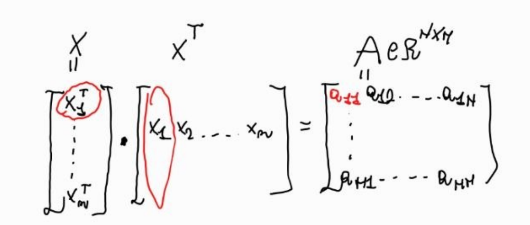
\includegraphics[width=0.8\textwidth]{_files/_images/mul1.png}
\caption{In questa immagine, si vede chiaramente, che facendo la moltiplicazioni fra le due matrici $X$ e $X^T$, si avrà ad esempio che l'elemento in posizione $(1,1)$ sarà $x_1^T x_1$
successivamente una volta fatto questo per tutti gli elementi, si applica la funzione SOFTMAX, che applica l'esponenziale al prodotto, e normalizza per riga.
Cioè è chiaramente quello che si fa nell'\textbf{equazione 3.7} per calcolare $a_{nm}$}
\end{figure}




Successivamente si moltiplica la matrice $A$ per la matrice $X$, quello che esce fuori è la matrice $Y$ dei vettori trasformati, dove la riga $n-esima$ conterrà $y_n^t$
\paragraph{Perchè esce fuori la matrice $Y$ ?}
Questo perchè ricorda la relazione di attenzione, ad esempio per $n$ = 1:
\begin{equation}
    y_1 = a_{11} \begin{pmatrix} x_{11} \\ x_{12} \\ \dots \\ x_{1D} \end{pmatrix} + a_{12} \begin{pmatrix} x_{21} \\ x_{22} \\ \dots \\ x_{2D} \end{pmatrix} + \dots + a_{1N} \begin{pmatrix} x_{N1} \\ x_{N2} \\ \dots \\ x_{ND} \end{pmatrix} 
\end{equation} 
Quindi il primo elemento del vettore $y_1$ è dato da:
\begin{equation}
    a_{11} x_{11} + a_{12} x_{21} + \dots + a_{1N} x_{N1}
\end{equation}
E infatti rivedendo la moltiplicazione fra matrici riga per colonna, fra $A$ e $X$, si ha:
\begin{equation}
    A = 
    \begin{pmatrix}
    a_{11} & a_{12} & \dots & a_{1N} \\
    a_{21} & a_{22} & \dots & a_{2N} \\
    \dots  \\
    a_{N1} & a_{N2} & \dots & a_{NN} 
    \end{pmatrix}
    X = 
    \begin{pmatrix}
    x_{11} & x_{12} & \dots & x_{1D} \\
    x_{21} & x_{22} & \dots & x_{2D} \\
    \dots \\
    x_{N1} & x_{N2} & \dots & x_{ND} 
    \end{pmatrix}
\end{equation}
Si ha che il primo elemento della matrice $y_{11}$ è proprio:
\begin{equation}
    a_{11} x_{11} + a_{12} x_{21} + \dots + a_{1N} x_{N1}
\end{equation}
Questo poi vale per tutti gli elementi di $y_1$ che sarà formato dalla prima riga.



\newpage

\section{Parametri di Rete (\textit{Network Parameters})} La formulazione base della Dot-Product Self-Attention soffre di due gravi limitazioni architetturali :
\begin{enumerate}
\item È una trasformazione totalmente fissa e deterministica, priva di parametri appresi; di conseguenza, non possiede alcuna capacità di apprendere dai dati. Tutte le feature all'interno di un vettore token $x\_n$ giocano esattamente lo stesso ruolo nel determinare la similarità. Sarebbe invece opportuno che la rete avesse la flessibilità di focalizzarsi maggiormente su determinate feature rispetto ad altre .
\end{enumerate}

Un tentativo primordiale per introdurre parametri consiste nell'applicare una trasformazione lineare $\tilde{X} = X U$, dove $U \in \mathbb{R}^{D \times D}$ è una matrice di pesi apprendibili. Ciò condurrebbe alla forma $Y = \text{Softmax}[X U U^\top X^\top] X U$. Tuttavia, tale formulazione rende la matrice degli argomenti del softmax $X U U^\top X^\top$ strettamente \emph{simmetrica}.

La simmetria è una proprietà indesiderabile per l'attenzione: le relazioni concettuali nel mondo reale sono intrinsecamente asimmetriche. Ad esempio, la parola ``scalpello'' deve essere fortemente associata alla parola ``utensile'' (poiché ogni scalpello è un utensile), ma la parola ``utensile'' deve essere solo debolmente associata a ``scalpello'' (esistendo molti altri tipi di utensili).

\subsection{Matrici di Proiezione Indipendenti $W^{(q)}$, $W^{(k)}$, $W^{(v)}$}
Per superare la simmetria e dotare il modello della massima espressività, si introducono tre trasformazioni lineari distinte e indipendenti per le Query, le Keys e i Values:
\begin{align}
Q &= X W^{(q)} \label{eq:proj_q} \\
K &= X W^{(k)} \label{eq:proj_k} \\
V &= X W^{(v)} \label{eq:proj_v}
\end{align}
dove $W^{(q)}, W^{(k)}, W^{(v)}$ sono matrici di parametri apprendibili durante la fase di addestramento:
\begin{itemize}
    \item $W^{(k)} \in \mathbb{R}^{D \times D_k}$, dove $D_k$ è la dimensione del vettore Key;
    \item $W^{(q)} \in \mathbb{R}^{D \times D_k}$, affinché i vettori Query abbiano la stessa dimensione $D_k$ dei vettori Key per poterne calcolare il prodotto scalare. Una scelta tipica è $D_k = D$.
    \item $W^{(v)} \in \mathbb{R}^{D \times D_v}$, dove $D_v$ rappresenta la dimensione dei vettori Value e dell'output. Ponendo $D_v = D$, l'output mantiene la stessa dimensione dell'input, facilitando l'introduzione di connessioni residuali e lo stacking di più livelli.
\end{itemize}

L'equazione dell'attenzione parametrizzata diventa quindi:
\begin{equation}
Y = \text{Softmax}\left[ Q K^\top \right] V
\end{equation}
in cui $Q K^\top \in \mathbb{R}^{N \times N}$ misura la matrice delle similarità incrociate asimmetriche tra tutti i token Query e Key, e $Y \in \mathbb{R}^{N \times D_v}$.



\begin{figure}[h]
\centering
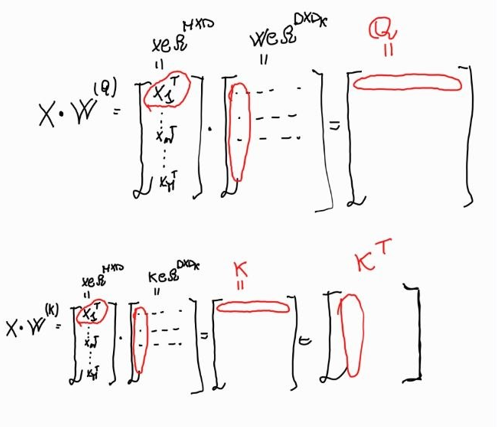
\includegraphics[width=0.4\textwidth]{_files/_images/mul2.png}
\caption{Quindi ora, ogni riga di $Q$, rappresenta \textbf{la query del vettore, cioè quello che il vettore cerca, la colonna di $K^T$} rappresenta quello che il vettore vuole "dichiarare" o rappresenta.
Il prodotto fra riga e colonna è come fare $x_n^T xn$ solo che in questo caso abbiamo matrici di peso apprendibili e quindi rappresentano precisamente quello che il vettore cerca e quello che vuole rappresentare, poi facendo la SOFTMAX (cioè esponenziale e calcolando per riga), dopo aver calcolato tutti gli elementi,
si avrà una matrice quadrata $N x N$, di coefficienti $a_{i,j}$, quei coefficienti si moltiplicano, per la matrice $V$ (che alla fine per ogni riga avremo il vettore $y_n$ di \textbf{l'equazione 3.3}), che rappresenta i valori veri, dopo questa moltiplicazione si avrà $Y$, la matrice finale}

\end{figure}


\newpage




\subsection{Confronto con le Reti Neurali Convenzionali}
Nelle reti neurali tradizionali, i percorsi di segnale moltiplicano le attivazioni per pesi sinaptici $W_{ij}$ fissi ed indipendenti dai dati correnti. Nel Transformer, al contrario, le attivazioni vengono moltiplicate per coefficienti di attenzione $a_{nm}$ che sono \emph{funzioni dinamiche dipendenti dai dati di input specifici}. Se un coefficiente $a_{nm}$ si annulla per un dato input, il segnale proveniente dal token $m$ viene completamente ignorato nella costruzione dell'output $n$.

\section{Self-Attention Scalata (\textit{Scaled Self-Attention})}
Sussiste un'ulteriore criticità di natura numerica. Quando la dimensione $D_k$ dei vettori Key e Query diventa elevata, il prodotto scalare $q^\top k$ tende ad assumere valori di magnitudo molto grande.

Poiché la funzione Softmax contiene esponenziali $\exp(q^\top k)$, valori di input molto grandi spingono l'attivazione nelle regioni estreme della funzione, dove la derivata è quasi nulla. Questo fenomeno causa la \textbf{saturazione dei gradienti} (\textit{vanishing gradient problem}), rendendo l'addestramento tramite backpropagation estremamente lento o instabile.

\subsection{Derivazione del Fattore di Scala $\sqrt{D_k}$}
Ipotizziamo che le componenti dei vettori Query e Key siano variabili casuali indipendenti a media nulla e varianza unitaria: $\mathbb{E}[q_i] = 0, \text{Var}(q_i) = 1$ e $\mathbb{E}[k_i] = 0, \text{Var}(k_i) = 1$.
Il loro prodotto scalare è dato da $q^\top k = \sum_{i=1}^{D_k} q_i k_i$. La varianza del prodotto di due variabili indipendenti a media zero è $1$, per cui la varianza della somma di $D_k$ termini indipendenti risulta:
\begin{equation}
\text{Var}\left(q^\top k\right) = D_k
\end{equation}
La deviazione standard del prodotto scalare è quindi pari a $\sqrt{D_k}$.

Per scalare la varianza riportandola all'unità (indipendentemente dalla dimensione $D_k$), si divide il prodotto scalare $Q K^\top$ per il fattore di scala $\sqrt{D_k}$.

\subsection{Formula Finale della Scaled Dot-Product Self-Attention}
Si perviene alla formulazione definitiva del livello di attenzione:
\begin{equation}
\text{Attention}(Q, K, V) \equiv \text{Softmax}\left[ \frac{Q K^\top}{\sqrt{D_k}} \right] V \label{eq:scaled_dot_product_attention}
\end{equation}

L'algoritmo formale per il calcolo della \textit{Scaled Dot-Product Self-Attention} è strutturato come segue:

\begin{tcolorbox}[colback=gray!5!white,colframe=gray!75!black,title=Algoritmo 12.1: Scaled Dot-Product Self-Attention]
\textbf{Input:} Insieme di token $X \in \mathbb{R}^{N \times D}$; Matrici di peso $W^{(q)}, W^{(k)} \in \mathbb{R}^{D \times D_k}$ e $W^{(v)} \in \mathbb{R}^{D \times D_v}$.\\
\textbf{Output:} $\text{Attention}(Q, K, V) \in \mathbb{R}^{N \times D_v}$.
\begin{enumerate}
    \item Calcola la matrice delle Query: $Q = X W^{(q)} \in \mathbb{R}^{N \times D_k}$
    \item Calcola la matrice delle Keys: $K = X W^{(k)} \in \mathbb{R}^{N \times D_k}$
    \item Calcola la matrice dei Values: $V = X W^{(v)} \in \mathbb{R}^{N \times D_v}$
    \item \textbf{return} $\text{Attention}(Q, K, V) = \text{Softmax}\left[ \frac{Q K^\top}{\sqrt{D_k}} \right] V$
\end{enumerate}
\end{tcolorbox}

\section{Attenzione Multi-Testa (\textit{Multi-Head Attention})}
Un singolo livello di attenzione (detto \textbf{testa di attenzione} o \textit{attention head}) permette all'output di prestare attenzione a un determinato pattern di relazioni dipendente dai dati. Tuttavia, all'interno della medesima sequenza possono coesistere simultaneamente \emph{molteplici pattern di relazioni differenti e rilevanti}. Ad esempio, nel linguaggio naturale, un pattern potrebbe essere legato alle concordanze grammaticali dei tempi verbali, mentre un altro potrebbe riguardare le relazioni semantiche del vocabolario.

Affidarsi a una sola testa di attenzione rischia di produrre un'indesiderata mediazione (\textit{averaging}) tra questi diversi effetti. Si introducono pertanto $H$ \textbf{teste di attenzione in parallelo}.

\subsection{Formulazione Matematica dell'Attenzione Multi-Testa}
Ciascuna testa $h \in \{1, \dots, H\}$ possiede le proprie matrici di proiezioni apprendibili $W_h^{(q)}, W_h^{(k)}, W_h^{(v)}$ ed effettua in modo indipendente il calcolo dell'attenzione scalata:
\begin{align}
Q_h &= X W_h^{(q)}, \quad K_h = X W_h^{(k)}, \quad V_h = X W_h^{(v)} \\
H_h &= \text{Attention}(Q_h, K_h, V_h) \in \mathbb{R}^{N \times D_v}
\end{align}

Le matrici risultanti $H_1, H_2, \dots, H_H$ vengono poi \textbf{concatenate} orizzontalmente in un'unica matrice di dimensione $N \times (H D_v)$. Il risultato concatenato viene infine proiettato linearmente tramite una matrice di output $W^{(o)} \in \mathbb{R}^{(H D_v) \times D}$:
\begin{equation}
Y(X) = \text{Concat}\left[ H_1, H_2, \dots, H_H \right] W^{(o)} \label{eq:mha_concat}
\end{equation}

Per fare in modo che la dimensione dell'output finale $Y$ sia identica alla dimensione dell'input $X \in \mathbb{R}^{N \times D}$, si sceglie tipicamente:
\begin{equation}
D_v = \frac{D}{H} \implies H D_v = D
\end{equation}
In questo modo, la dimensione complessiva del calcolo rimane comparabile a quella di un'attenzione singola a piena dimensione.



L'algoritmo complessivo per l'Attenzione Multi-Testa è formalizzato di seguito:


\begin{tcolorbox}[colback=gray!5!white,colframe=gray!75!black,title=Algoritmo 12.2: Multi-Head Attention]
\textbf{Input:} Insieme di token $X \in \mathbb{R}^{N \times D}$; Matrici di peso Query $\{W_1^{(q)}, \dots, W_H^{(q)}\} \in \mathbb{R}^{D \times D_k}$; Matrici Key $\{W_1^{(k)}, \dots, W_H^{(k)}\} \in \mathbb{R}^{D \times D_k}$; Matrici Value $\{W_1^{(v)}, \dots, W_H^{(v)}\} \in \mathbb{R}^{D \times D_v}$; Matrice di Output $W^{(o)} \in \mathbb{R}^{(H D_v) \times D}$.\\
\textbf{Output:} $Y \in \mathbb{R}^{N \times D}$.
\begin{enumerate}
    \item \textbf{for} $h = 1, \dots, H$ \textbf{do}
    \item \quad $Q_h = X W_h^{(q)}$, $\quad K_h = X W_h^{(k)}$, $\quad V_h = X W_h^{(v)}$
    \item \quad $H_h = \text{Attention}(Q_h, K_h, V_h) \in \mathbb{R}^{N \times D_v}$
    \item \textbf{end for}
    \item $H = \text{Concat}\left[ H_1, \dots, H_H \right] \in \mathbb{R}^{N \times (H D_v)}$
    \item \textbf{return} $Y(X) = H W^{(o)}$
\end{enumerate}
\end{tcolorbox}

\textbf{In questo senso, la notazione $Y(X)$, vuol dire che $Y$ è prodotta in output, quando in input ha $X$.}.

Nel nostro caso $Y(X) = Y$.
\begin{center}
    Y è il nome dell'output; \(Y(X)\) enfatizza che quell'output è una funzione dell'input X
\end{center}


\section{Livello Transformer (\textit{Transformer Layer})}
L'attenzione multi-testa costituisce il nucleo centrale del Transformer. Tuttavia, per costruire reti profonde ed espressive, occorre impilare più livelli di attenzione uno sopra l'altro.

\subsection{Connessioni Residuali e Layer Normalization}
Per garantire un flusso di gradiente stabile durante l'addestramento di reti molto profonde, si introducono \textbf{connessioni residuali} (\textit{residual connections}) che scavalcano il blocco di attenzione. A queste si associa la \textbf{Layer Normalization} (\textit{LayerNorm}):

\begin{equation}
Z = \text{LayerNorm}\left[ Y(X) + X \right] \label{eq:post_norm}
\end{equation}
dove $Y(X)$ è l'output dell'attenzione multi-testa \eqref{eq:mha_concat}. La formulazione \eqref{eq:post_norm} prende il nome di \textbf{Post-Norm}.

Nelle implementazioni moderne si preferisce talvolta la variante \textbf{Pre-Norm}, in cui la normalizzazione viene applicata prima del blocco di attenzione:
\begin{equation}
Z = Y(X') + X, \quad \text{con } X' = \text{LayerNorm}[X] \label{eq:pre_norm}
\end{equation}
\textbf{Si chiama Pre-Norm}, perchè la normalizzazione avviene prima del layer di attenzione.
La configurazione Pre-Norm facilita un'ottimizzazione più stabile nelle fasi iniziali dell'addestramento. In entrambi i casi, la matrice intermedia $Z$ mantiene la dimensionalità $N \times D$.

\subsection{Il Ruolo della Rete Non Lineare MLP}
Il solo meccanismo di attenzione presenta un forte limite espressivo: gli output $Y$ generati dall'attenzione sono limitati ad essere \emph{combinazioni lineari} dei vettori Value $V$, i quali sono a loro volta trasformazioni lineari degli input $X$. La non-linearità entra soltanto attraverso i coefficienti scalari forniti dal Softmax. Di conseguenza, i vettori di output rimangono vincolati a risiedere nel sottospazio lineare generato dagli input.

Per rompere questa limitazione e aumentare l'espressività della rete, l'output $Z$ viene post-elaborato applicando a ciascuna riga (ovvero a ciascun token in modo del tutto indipendente e condiviso) una rete neurale \textbf{Perceptron Multistrato} (MLP) non lineare con $D$ ingressi e $D$ uscite:
\begin{equation}
\text{MLP}[Z]
\end{equation}
Tipicamente, l'MLP è costituito da una rete fully-connected a due strati con funzioni di attivazione non lineari di tipo \text{ReLU} o \text{GELU} negli strati nascosti.

Anche il blocco MLP viene avvolto da una connessione residuale e da Layer Normalization:
\begin{equation}
\tilde{X} = \text{LayerNorm}\left[ \text{MLP}[Z] + Z \right] \label{eq:transformer_layer_final}
\end{equation}
(ovvero nella variante Pre-Norm: $\tilde{X} = \text{MLP}(Z') + Z$ con $Z' = \text{LayerNorm}[Z]$).

\subsection{Struttura Complessiva dell'Algoritmo}
L'architettura completa di un generico \textit{Transformer Layer} è riassunta nell'Algoritmo 12.3:

\begin{tcolorbox}[colback=gray!5!white,colframe=gray!75!black,title=Algoritmo 12.3: Transformer Layer]
\textbf{Input:} Insieme di token $X \in \mathbb{R}^{N \times D}$; Parametri del livello di Attenzione Multi-Testa; Parametri della rete feed-forward MLP.\\
\textbf{Output:} $\tilde{X} \in \mathbb{R}^{N \times D}$.
\begin{enumerate}
    \item Applica l'attenzione multi-testa con connessione residuale e LayerNorm:
    \begin{equation*}
    Z = \text{LayerNorm}\left[ Y(X) + X \right] \quad \text{(dove } Y(X) \text{ è dato dall'Algoritmo 12.2)}
    \end{equation*}
    \item Applica la rete feed-forward MLP condivisa con connessione residuale e LayerNorm:
    \begin{equation*}
    \tilde{X} = \text{LayerNorm}\left[ \text{MLP}[Z] + Z \right]
    \end{equation*}
    \item \textbf{return} $\tilde{X}$
\end{enumerate}
\end{tcolorbox}


\newpage


\begin{figure}[h]
    \centering
    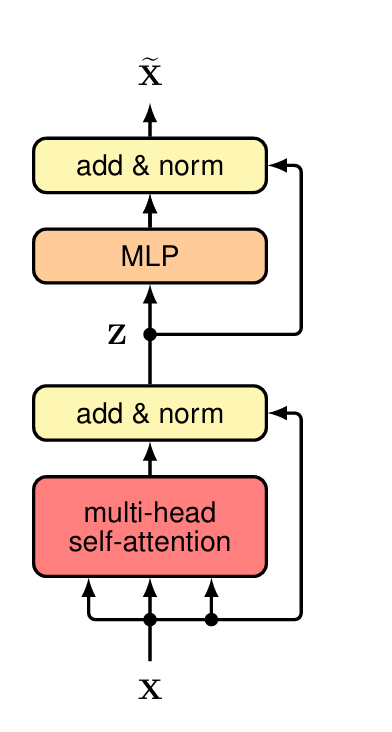
\includegraphics[width=0.4\textwidth]{_files/_images/transformer.png}
    \caption{Archittetura di un layer di un Transformer}
    \label{fig:GPT}
\end{figure}



Un'architettura Transformer completa consiste nello stacking sequenziale di $L$ livelli identici di questo tipo. Ciascun livello possiede le proprie matrici di peso e bias apprendibili indipendenti (non vi è condivisione di parametri tra livelli differenti).


\section{Codifica Posizionale (\textit{Positional Encoding})}
Esiste una proprietà fondamentale dell'architettura Transformer formulata finora che rappresenta sia una grande forza che un limite critico.

\subsection{Il Problema dell'Equivarianza alle Permutazioni}
Poiché le matrici di peso $W_h^{(q)}, W_h^{(k)}, W_h^{(v)}$ dell'attenzione e la successiva rete MLP sono condivise in modo del tutto identico tra tutti i token, il Transformer possiede la proprietà di essere \textbf{equivariante rispetto alle permutazioni degli input}.

\begin{definition}{Equivarianza alle Permutazioni}
Sia $P$ una matrice di permutazione delle righe. Se si applica una permutazione $P X$ alla matrice di input $X$, l'output del Transformer Layer risulterà esattamente permutato dalla medesima matrice $P$:
\begin{equation}
\text{TransformerLayer}[P X] = P \, \text{TransformerLayer}[X]
\end{equation}
\end{definition}

In altre parole, il Transformer è intrinsecamente un modello che elabora \emph{insiemi non ordinati} (\textit{un-ordered sets}) di vettori. Tuttavia, per dati sequenziali come il linguaggio naturale, l'ordine dei token è assolutamente fondamentale per definire il significato. Ad esempio, le due frasi:
\begin{center}
\textit{``Il cibo era cattivo, per niente buono.''} \quad e \quad \textit{``Il cibo era buono, per niente cattivo.''}
\end{center}
contengono esattamente gli stessi token, ma esprimono significati opposti a causa del differente ordine delle parole.

Per elaborare sequenze, occorre quindi iniettare l'informazione sull'ordine dei token all'interno della rete.

\subsection{Somma vs Concatenazione della Codifica Posizionale}
Invece di modificare l'architettura della rete (il che distruggerebbe la parallellizzabilità dell'attenzione), si sceglie di codificare la posizione direttamente nei dati di input.

Per ciascuna posizione \(n \in \{1, \dots, N\}\), si definisce un vettore di \textbf{codifica posizionale} \(r_n\). Si pongono due alternative per combinare \(r_n\) con il vettore di embedding del token \(x_n\):
\begin{enumerate}
    \item \textbf{Concatenazione:} \([x_n; r_n]\). Aumenterebbe la dimensione dell'input da \(D\) a \(D + D_{pos}\), aumentando la dimensione di tutte le matrici di attenzione e quindi il costo computazionale di tutti i livelli successivi.
    \item \textbf{Somma (Addizione):}
    \begin{equation}
    \tilde{x}_n = x_n + r_n
    \end{equation}
    richiedendo che il vettore di posizione \(r_n \in \mathbb{R}^D\) abbia esattamente la stessa dimensionalità del vettore token \(x_n\).
\end{enumerate}

\begin{observation}{Perché l'Addizione non Corrompe l'Informazione del Token?}
Potrebbe sembrare che sommare l'informazione di posizione al vettore del token corrompa la rappresentazione del token stesso. L'intuizione matematica risiede nel fatto che, in spazi ad altissima dimensione (\(D\) grande), due vettori casuali non correlati tendono ad essere \textbf{quasi ortogonali}. Di conseguenza, la rete è in grado di separare ed elaborare in modo indipendente l'identità del token e la sua posizione. Inoltre, la presenza di connessioni residuali in ogni livello previene la perdita dell'informazione posizionale lungo la profondità della rete.
\end{observation}

\subsection{Proprietà di una Codifica Posizionale Ideale}
Un meccanismo di codifica posizionale ideale deve soddisfare quattro requisiti chiave:
\begin{enumerate}
    \item Fornire una rappresentazione unica per ciascuna posizione \(n\);
    \item Mantenere i valori limitati in magnitudo (per evitare sbilanciamenti numerici con \(x_n\));
    \item Generalizzare a sequenze di lunghezza maggiore rispetto a quelle osservate durante l'addestramento;
    \item Permettere di esprimere le posizioni relative tra due token (ovvero la distanza \(k\) tra la posizione \(n\) e la posizione \(n+k\)) in modo coerente ed indipendente dalla posizione assoluta \(n\).
\end{enumerate}

\subsection{Codifica Posizionale Sinusoidale (\textit{Sinusoidal Positional Encoding})}
Vaswani et al. (2017) hanno introdotto una celebre codifica deterministica basata su funzioni trigonometriche ad onde con frequenze crescenti. Per una posizione \(n \in \{1, \dots, N\}\) e un indice di feature \(i \in \{0, \dots, D-1\}\), la componente \(i\)-esima del vettore \(r_n\) è definita come:
\begin{equation}
r_{ni} = \begin{cases}
\sin\left( \frac{n}{L^{i/D}} \right) & \text{se } i \text{ è pari} \\[8pt]
\cos\left( \frac{n}{L^{(i-1)/D}} \right) & \text{se } i \text{ è dispari}
\end{cases} \label{eq:sinusoidal_pe}
\end{equation}
dove \(L\) è una costante di scala di frequenza (tipicamente \(L = 10000\)).

\begin{observation}{Proprietà delle Funzioni Sinusoidali}
\begin{itemize}
    \item Tutti gli elementi del vettore \(r_n\) sono limitati nell'intervallo \([-1, 1]\).
    \item Le componenti alternano funzioni seno e coseno con lunghezze d'onda gradualmente crescenti lungo le dimensioni dell'embedding. Ciò ricorda la rappresentazione dei numeri binari, in cui il bit meno significativo varia ad altissima frequenza e i bit successivi variano con frequenze via via dimezzate.
    \item \textbf{Rappresentazione delle Posizioni Relative:} Per qualsiasi offset fisso \(k\), la codifica posizionale alla posizione \(n+k\) può essere espressa come una \emph{trasformazione lineare} della codifica alla posizione \(n\), con un coefficiente di matrice che dipende unicamente dal valore dell'offset \(k\) e non dalla posizione assoluta \(n\). Tale proprietà discende direttamente dalle identità trigonometriche di addizione:
    \begin{align*}
    \sin(\alpha + \beta) &= \sin(\alpha)\cos(\beta) + \cos(\alpha)\sin(\beta) \\
    \cos(\alpha + \beta) &= \cos(\alpha)\cos(\beta) - \sin(\alpha)\sin(\beta)
    \end{align*}
\end{itemize}
\end{observation}

\subsection{Codifiche Posizionali Apprese (\textit{Learned Positional Encodings})}
Un'alternativa ampiamente utilizzata consiste nell'impiegare \textbf{codifiche posizionali apprese}: si associa a ciascuna posizione \(n\) un vettore di parametri apprendibili \(r_n \in \mathbb{R}^D\), ottimizzato congiuntamente al resto del modello durante la fase di addestramento.

Sebbene questo approccio eviti la progettazione euristica di funzioni trigonometriche, esso presenta un limite fondamentale: \emph{non è in grado di generalizzare a sequenze di lunghezza superiore a quelle osservate durante l'addestramento}, poiché i vettori corrispondenti a posizioni non viste non sono mai stati aggiornati dai gradienti. Pertanto, le codifiche apprese sono adatte principalmente quando la lunghezza delle sequenze rimane approssimativamente costante tra addestramento e inferenza.

\subsubsection{Gerarchia dei Language Models}

Nel contesto della \textit{Generative AI} si incontrano frequentemente i termini \textbf{Language Model (LM)}, \textbf{Generative Language Model} e \textbf{Large Language Model (LLM)}. Questi concetti sono collegati tra loro, ma descrivono aspetti differenti di un modello.

Una rappresentazione intuitiva è:

\begin{equation}
\text{Language Model}
\supseteq
\text{Generative Language Model}
\supseteq
\text{Large Language Model (LLM)}
\end{equation}

Questa rappresentazione deve però essere interpretata con cautela: il termine \textit{LLM} non identifica semplicemente una particolare funzione del modello, ma indica principalmente un \textbf{Language Model di grande scala}. Il termine ``generative'', invece, descrive la capacità del modello di generare nuove sequenze linguistiche.

\subsubsection{Language Model}

Un \textbf{Language Model (LM)} è un modello che descrive la distribuzione di probabilità delle sequenze di token appartenenti a un linguaggio.

Consideriamo una sequenza di token:

\begin{equation}
x_1,x_2,\ldots,x_n.
\end{equation}

Il Language Model cerca di modellare la probabilità congiunta:

\begin{equation}
P(x_1,x_2,\ldots,x_n).
\end{equation}

Grazie alla \textbf{chain rule della probabilità}, questa probabilità può essere scomposta nel prodotto:

\begin{equation}
P(x_1,\ldots,x_n)
\prod_{i=1}^{n}
P(x_i\mid x_1,\ldots,x_{i-1}).
\end{equation}

Quindi, in particolare, il modello può stimare la probabilità del prossimo token conoscendo quelli precedenti:

\begin{equation}
P(x_i\mid x_1,\ldots,x_{i-1}).
\end{equation}

\paragraph{Esempio.}

Supponiamo di avere la sequenza:

\begin{center}
\texttt{Il gatto è}
\end{center}

Il Language Model può stimare probabilità come:

\begin{align}
P(\texttt{seduto}\mid \texttt{Il gatto è}) &= 0.35,\
P(\texttt{rosso}\mid \texttt{Il gatto è}) &= 0.10,\
P(\texttt{grande}\mid \texttt{Il gatto è}) &= 0.08.
\end{align}

In questo modo il modello rappresenta le regolarità statistiche presenti nel linguaggio.

\begin{warning}
Un Language Model non deve necessariamente essere interpretato come un modello che ``scrive testo''. Il concetto fondamentale è che \textbf{modella probabilisticamente il linguaggio}, cioè assegna probabilità alle sequenze o ai token condizionati al contesto.
\end{warning}

\subsubsection{Generative Language Model}

Un \textbf{Generative Language Model} è un Language Model che viene utilizzato per \textbf{generare nuove sequenze di testo}.

Nel caso di un modello autoregressivo, la generazione avviene tipicamente un token alla volta.

Supponiamo di avere:

\begin{center}
\texttt{Il gatto è}
\end{center}

Il modello calcola una distribuzione di probabilità sul prossimo token:

\begin{equation}
P(x_{t+1}\mid x_1,\ldots,x_t).
\end{equation}

Supponiamo che venga scelto il token:

\begin{center}
\texttt{seduto}.
\end{center}

La sequenza diventa:

\begin{center}
\texttt{Il gatto è seduto}
\end{center}

A questo punto il modello calcola nuovamente la distribuzione del prossimo token:

\begin{equation}
P(x_{t+2}\mid x_1,\ldots,x_t,\texttt{seduto}).
\end{equation}

Potrebbe quindi generare:

\begin{center}
\texttt{Il gatto è seduto sul}
\end{center}

e continuare nello stesso modo.

Possiamo quindi schematizzare il processo come:

\begin{equation}
\text{contesto}
\longrightarrow
\text{distribuzione sul prossimo token}
\longrightarrow
\text{scelta del token}
\longrightarrow
\text{nuovo contesto}.
\end{equation}

Ad esempio:

\begin{center}
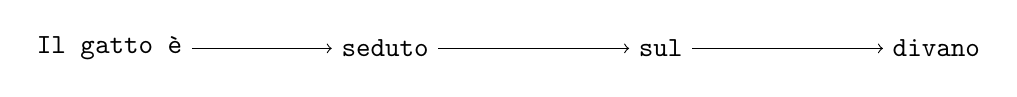
\begin{tikzpicture}[node distance=1.5cm]
\node (a) {\texttt{Il gatto è}};
\node (b) [right of=a, xshift=2cm] {\texttt{seduto}};
\node (c) [right of=b, xshift=2cm] {\texttt{sul}};
\node (d) [right of=c, xshift=2cm] {\texttt{divano}};

\draw[->] (a) -- (b);
\draw[->] (b) -- (c);
\draw[->] (c) -- (d);
\end{tikzpicture}
\end{center}

Il modello costruisce quindi progressivamente una nuova sequenza linguistica.

\subsubsection{Large Language Model (LLM)}

Un \textbf{Large Language Model (LLM)} è un Language Model caratterizzato da una \textbf{grande scala}.

Il termine ``Large'' si riferisce principalmente alla dimensione e alla complessità del modello. In particolare, gli LLM moderni possono avere:

\begin{itemize}
\item un numero molto elevato di parametri;
\item enormi quantità di dati utilizzati durante il training;
\item elevati costi computazionali per l'addestramento;
\item una notevole capacità di rappresentare strutture e regolarità del linguaggio.
\end{itemize}

Il termine LLM, quindi, non descrive direttamente il meccanismo con cui il modello genera il testo. Descrive principalmente la \textbf{scala} del Language Model.

Per esempio, GPT, Llama e altri modelli linguistici moderni appartengono alla categoria degli LLM.

\subsubsection{Come sono collegati i tre concetti?}

Possiamo ora riassumere il rapporto tra i termini:

\begin{center}
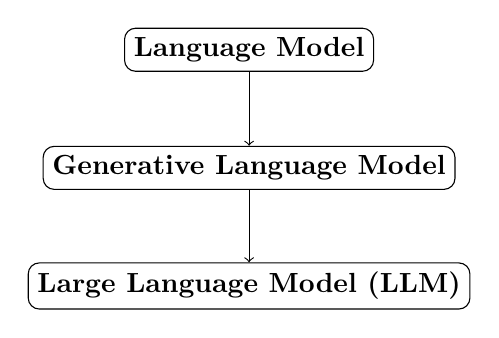
\begin{tikzpicture}[node distance=1.5cm]
\node (lm) [draw, rounded corners] {\textbf{Language Model}};
\node (glm) [draw, rounded corners, below of=lm] {\textbf{Generative Language Model}};
\node (llm) [draw, rounded corners, below of=glm] {\textbf{Large Language Model (LLM)}};

\draw[->] (lm) -- (glm);
\draw[->] (glm) -- (llm);
\end{tikzpicture}
\end{center}

Tuttavia, è più preciso pensare a queste caratteristiche come a \textbf{dimensioni differenti}:

\begin{itemize}
\item \textbf{Language Model}: indica che il modello è progettato per modellare il linguaggio;
\item \textbf{Generative}: indica che il modello viene utilizzato per generare nuove sequenze linguistiche;
\item \textbf{Large}: indica che il modello ha una grande scala in termini di parametri, dati e capacità computazionale.
\end{itemize}

Pertanto, un modello può essere contemporaneamente:

\begin{equation}
\boxed{
\text{Language Model}
+
\text{Generative}
+
\text{Large}
}
\end{equation}

e in questo caso parliamo tipicamente di un \textbf{Generative LLM}.

\subsubsection{Dove si colloca il Transformer?}

Un'ulteriore fonte di confusione è il termine \textbf{Transformer}.

Il Transformer \textbf{non è una categoria di Language Model}. È invece un'\textbf{architettura di rete neurale} che può essere utilizzata per costruire Language Models.

Possiamo quindi distinguere i diversi livelli:

\begin{center}
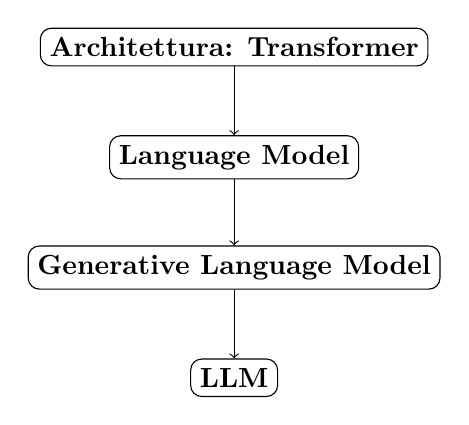
\begin{tikzpicture}[node distance=1.4cm]
\node (t) [draw, rounded corners] {\textbf{Architettura: Transformer}};
\node (lm) [draw, rounded corners, below of=t] {\textbf{Language Model}};
\node (gen) [draw, rounded corners, below of=lm] {\textbf{Generative Language Model}};
\node (llm) [draw, rounded corners, below of=gen] {\textbf{LLM}};

\draw[->] (t) -- (lm);
\draw[->] (lm) -- (gen);
\draw[->] (gen) -- (llm);
\end{tikzpicture}
\end{center}

Questa rappresentazione è utile per capire che stiamo parlando di concetti diversi.

Il \textbf{Transformer} risponde alla domanda:

\begin{center}
\textit{``Come è costruita l'architettura del modello?''}
\end{center}

Il \textbf{Language Model} risponde invece alla domanda:

\begin{center}
\textit{``Che tipo di problema linguistico stiamo modellando?''}
\end{center}

Il termine \textbf{Generative} indica:

\begin{center}
\textit{``Il modello viene utilizzato per generare nuove sequenze?''}
\end{center}

Infine, il termine \textbf{Large} indica:

\begin{center}
\textit{``Quanto è grande il modello?''}
\end{center}

\subsubsection{Schema riassuntivo}

La distinzione può essere riassunta nella seguente tabella:

\begin{center}
\begin{tabular}{|c|c|}
\hline
\textbf{Termine} & \textbf{Cosa descrive?} \\
\hline
Language Model & Modella il linguaggio \\
\hline
Generative Language Model & Genera nuove sequenze linguistiche \\
\hline
LLM & Language Model di grande scala \\
\hline
Transformer & Architettura neurale utilizzabile per costruire il modello \\
\hline
\end{tabular}
\end{center}

Per esempio, possiamo descrivere un modello come GPT, in maniera semplificata, dicendo che è un:

\begin{equation}
\boxed{
\text{LLM generativo basato sull'architettura Transformer}
}
\end{equation}

Quindi è importante non confondere i livelli:

\begin{center}
\textbf{Transformer}
\(\quad\rightarrow\quad\)
\text{architettura}
\end{center}

\begin{center}
\textbf{Language Model}
\(\quad\rightarrow\quad\)
\text{modello del linguaggio}
\end{center}

\begin{center}
\textbf{Generative}
\(\quad\rightarrow\quad\)
\text{capacità/modalità di generazione}
\end{center}

\begin{center}
\textbf{Large}
\(\quad\rightarrow\quad\)
\text{scala del modello}
\end{center}




